\documentclass[a4paper,12pt,openright,oneside]{book}

% Enables Portuguese Brasil
\usepackage[portuguese]{babel}

% Enables code listing
\usepackage{listings}
%--------------------------------------

\usepackage{xcolor}

%--------------------------------------

\usepackage[T1]{fontenc}
\usepackage[utf8]{inputenc}

\usepackage[figuresright]{rotating}
\usepackage{amsthm}
\usepackage{graphics}
\usepackage{amssymb}
\usepackage{graphicx}
\usepackage{fancybox}
\usepackage{amsmath}
\usepackage{picinpar}
\usepackage{colortbl}
\usepackage{wasysym}
\usepackage{txfonts}
\usepackage{pb-diagram}
\usepackage{relsize}
\usepackage{tikz}
	\usetikzlibrary{calc}
	\usetikzlibrary{datavisualization}
	\usetikzlibrary{positioning}
	\usetikzlibrary{mindmap}
	\usetikzlibrary{snakes}
	\usetikzlibrary{shapes}
	\usetikzlibrary{decorations.pathreplacing}
	\usetikzlibrary{spy}
	\usetikzlibrary{backgrounds}
	\usetikzlibrary{patterns}
\usepackage{pgfplots}
\usepackage{pgfplotstable}
	\pgfplotsset{compat=newest}
	\usepgfplotslibrary{units}
\usepackage{subfigure}
\usepackage{algorithm}
\usepackage{algorithmic}
\usepackage{verbatim}
\usepackage{wrapfig}
\usepackage{array}
\usepackage{calc}
\usepackage[T1]{fontenc}
\usepackage{times}
\usepackage{indentfirst}        % indenta primeiro par�grafo
\usepackage{fancyhdr}
\usepackage{pifont}
\usepackage{textcomp}      % \texttrademark
\usepackage{url}  
\usepackage{multirow}  
\usepackage[numbers]{natbib}
\usepackage{notoccite}
\usepackage{setspace}
\usepackage{array}
\usepackage{helvet}

\renewcommand{\familydefault}{\sfdefault}
\headheight 16pt
\setlength{\topmargin}{-15pt} % extra vert. space + at the top of header: 23pt
\setlength{\oddsidemargin}{0pt} % extra spc added at the left of odd page: 0pt
\setlength{\evensidemargin}{-12pt} % ext. spc added at the left of even pg: 59pt
\setlength{\textheight}{638pt} % height of the body: 592pt
\setlength{\textwidth}{483pt} % width of the body: 470pt
\pagestyle{fancyplain}
\renewcommand{\chaptermark}[1]{\markboth{#1}{}}
\renewcommand{\sectionmark}[1]{\markright{\thesection\ #1}}
\lhead[\fancyplain{}{\bfseries\thepage}]{\fancyplain{}{\bfseries\rightmark}}
\rhead[\fancyplain{}{\bfseries\leftmark}]{\fancyplain{}{\bfseries\thepage}}
\cfoot[\fancyplain{\bfseries\thepage}{}]{\fancyplain{\bfseries\thepage}{}}
\newenvironment{myenv}[1]
  {\begin{spacing}{#1}}
  {\end{spacing}}

%% Inicia o texto
\begin{document}
	%% Abrevia figuras e tabelas
	\thispagestyle{empty}
	\begin{center}
		\par \null
		\begin{figure}[H]
			\centering 
\includegraphics[angle=-90]{unesp.pdf}
		\end{figure} 
		\vspace{3cm}
		\fontsize{14}{\baselineskip} \selectfont
		{André Furlan} \\  
		\vspace{4.5cm}
		\onehalfspacing
		\fontsize{14}{\baselineskip} \selectfont
		Monografia de estudos especiais \\
		\vspace{7cm}
		\fontsize{14}{\baselineskip} \selectfont  
		{São José do Rio Preto}\\ \vspace{1.0pt} 
		{2019} 
	\end{center}

	%% *****ROSTO*****
	\newpage
	\thispagestyle{empty}
	\setcounter{page}{1}
	\begin{center}
		\vspace{4cm}
		\fontsize{14}{\baselineskip} \selectfont
		\vspace{30.0pt}
		{André Furlan} \\ \vspace{30.0pt}
		{Caracterização de \textit{voice spoofing} para fins de verificação de locutores com base na transformada wavelet e na análise paraconsistente de características} \\ \onehalfspacing \fontsize{14}{\baselineskip}
		\par \null
		\begin{flushright}
		\parbox{3.50in}{
			\fontsize{12}{\baselineskip} \selectfont \onehalfspacing
			Monografia apresentada para cumprimento da disciplina de estudos especiais do curso de Mestrado em Ciência da Computação, junto ao Programa de Pós-Graduação em Ciência da Computação, do Instituto de Biociências, Letras e Ciências Exatas da Universidade Estadual Paulista "Júlio de Mesquita Filho", Campus de São José do Rio Preto. \\ \vspace{1.0pt}
			{Orientador: Prof. Dr. Rodrigo Capobianco Guido } \\ \vspace{1.0pt}
		}
		\end{flushright}
		\fontsize{14}{\baselineskip} \selectfont
		\vspace{8.0cm}
		São José do Rio Preto, SP \\ \vspace{1.0pt}  
		2019
	\end{center}
	\newpage
	\thispagestyle{empty}

	%% *****APROVACAO*****
	\begin{center}
		\vspace{4cm}
		\fontsize{14}{\baselineskip} \selectfont
		\vspace{30.0pt}
		{André Furlan} \\ \vspace{30.0pt}
		{Caracterização de \textit{voice spoofing} para fins de verificação de locutores com base na transformada wavelet e na análise paraconsistente de características} \\ \onehalfspacing \fontsize{14}{\baselineskip} \selectfont
		\par \null
		\begin{flushright}
		\parbox{3.50in}{
			\fontsize{12}{\baselineskip} \selectfont \onehalfspacing
			Monografia apresentada para cumprimento da disciplina de estudos especiais do curso de Mestrado em Ciência da Computação, junto ao Programa de Pós-Graduação em Ciência da Computação, do Instituto de Biociências, Letras e Ciências Exatas da Universidade Estadual Paulista "Júlio de Mesquita Filho", Campus de São José do Rio Preto. \\ \vspace{1.0pt}
			{Orientador: Prof. Dr. Rodrigo Capobianco Guido } \\ \vspace{1.0pt}
		}
		\end{flushright}
		\fontsize{14}{\baselineskip} \selectfont
		Comissão Examinadora \\  \vspace{1.0pt}
	\end{center}

	\fontsize{14}{\baselineskip} \selectfont
	Professor Dr. Rodrigo Capobianco Guido \\ 
	UNESP - Campus de São José do Rio Preto \\
	Co-Orientador \\\\
	
	Professora Dra. Renata Spolon Lobato \\ 
	UNESP - Campus de São José do Rio Preto \\\\
	
	Professor Dr. Aleardo Manacero Júnior \\
	UNESP - Campus de São José do Rio Preto \\\\
	\vspace{3.0cm}

	\begin{center}
		São José do Rio Preto, SP  \\ \vspace{1.0pt}
		2019
	\end{center}

	%%
	%% *****Resumo*****
	%%

	%% Resumo/Abstract
	%% *****Resumo*****
	\setlength{\parindent}{0pt}
	\newpage \thispagestyle{empty}
	\vspace{1.5cm}
	\fontsize{12}{\baselineskip} \selectfont

	\begin{center}
		{\huge{\textbf{RESUMO}}}
	\end{center}

	\begin{myenv}{1.5}
		\fontsize{12}{\baselineskip} \selectfont \onehalfspacing
		\par \null
		\par \null
		\par Este documento constitui a monografia produzida como resultado dos estudos especiais realizados pelo autor visando promover um levantamento bibliográfico inicial do tema de sua dissertação de mestrado. Foram inclusas as descrições essenciais de 14 trabalhos científicos na área de \textit{voice spoofing detection}, acrescidos ainda, das direções que caracterizam o tema do trabalho em questão visando a monografia de qualificação.
		
		\par No capítulo 1 é feita uma breve introdução. Iniciando as revisões de conceitos apresenta-se a engenharia paraconsistente de características, filtros digitais \textit{wavelets}, amostragem,  quantização e o formato do arquivo \textit{wave} e caracterização dos processos de produção da voz humana no capítulo 2 seção 1, a seguir, na seção 2 deste mesmo capítulo apresenta-se a revisão bibliográfica inicial. Finalmente no capítulo 3 é mostrado um cronograma com os trabalhos já realizados e uma previsão da realização dos próximos.
		
	\end{myenv}

	%% Lista de figuras (gerada automaticamente)
	\cleardoublepage
	\pagenumbering{gobble}
	\listoffigures
	
	% Lista de tabelas (gerada automaticamente)
	\cleardoublepage
	\pagenumbering{gobble}
	\listoftables
	\frontmatter
	
	%% Lista de conte\'{u}do (sumário)
	\def\contentsname{Sumário} 
	\pagenumbering{gobble}
	\tableofcontents
	\cleardoublepage
	
	% \nobibintoc para bibliografia nao aparecer no indice
	%% Glossário (gerado automaticamente - veja entradas em cap1.tex)
	%\cleardoublepage
	%\renewcommand{\nomname}{Glossário}
	%\markboth{GLOSSáRIO}{GLOSSáRIO}
	%\addcontentsline{toc}{chapter}{\nomname}
	%\printnomenclature
	\mainmatter
	\setlength{\parindent}{1.25cm}

	\chapter{Introdução}
		\begin{myenv}{1.5}
			\setcounter{page}{12}
			\par Os sistemas de autenticação de usuário por voz e o processo de falseamento usando \textit{voice spoofing} é o tema de estudo que se pretende explorar. Um sistema de reconhecimento \textbf{idealmente} não deve se deixar enganar por, como exemplo, uma voz gravada, neste documento será apresentada uma revisão de conceitos que visa preparar as bases para a construção de métodos que reconheçam esse ataque.
			
			\par No capítulo 2 se realizará uma revisão dos seguintes conceitos:
			\begin{itemize}
				\item Engenharia paraconsistente.
				\item Filtros digitais usando wavelets.
				\item Caracterização dos processos de produção da voz humana.
				\item Amostragem, quantização, entre outros.
			\end{itemize}
			\par Em seguida apresentar-se-á uma revisão bibliográfica finalizando com o cronograma previsto.
		\end{myenv}

	\chapter{Revisão de Bibliográfica}
		\begin{myenv}{1.5}
			\section{Conceitos utilizados}
					\subsection{Engenharia paraconsistente de características}
						\par Dentro do processo de classificação frequentemente surge a questão:\\
						Os vetores de características criados proporcionam uma boa separação de classes?
						
						\par O método de cálculo do plano paraconsistente é uma ferramenta que pode ser usada para responder essa questão.
						
						\par O processo inicia-se após a aquisição dos vetores de características para cada classe ($C_n$) onde $n$ é o índice de cada uma delas. Se o número de classes presentes for, por exemplo, quatro então estas poderão ser representadas por $C_1, C_2, C_3, C_4$.
						\par Em seguida será necessário o cálculo de duas grandezas:
						
						\begin{itemize}
							\item A menor similaridade intraclasse ($\alpha$).
							\item A razão de sobreposição interclasse ($\beta$)
						\end{itemize}
					
						\par $\alpha$ indica o quanto de similaridade os dados têm entre si dentro de uma mesma classe, $\beta$ mostra a razão de sobreposição entre diferentes classes. Idealmente $\alpha$ deve ser maximizada e $\beta$ minimizada para um desempenho ótimo dos classificadores.
						
						\par Inicialmente é necessária a normalização dos vetores de características de forma que a soma de todos os seus valores seja um.
						
						\par Em seguida a obtenção de $\alpha$ se dá selecionando-se os maiores e os menores valores de cada uma das posições de todos os vetores de características de cada classe gerando assim um vetor para os valores maiores e outro para os menores.
						
						\par O \textbf{vetor de similaridade}$(svC_n)$ é obtido fazendo-se a diferença item-a-item dos maiores em relação aos menores.
						
						\par Finalmente e para cada classe é tirada a média dos valores de cada vetor de similaridade, $\alpha$ é o menor valor dentre essas médias.
						
						\par A figura \ref{fig:calculoalpha} ilustra este processo.
						
						\begin{figure}[h]
							\centering
							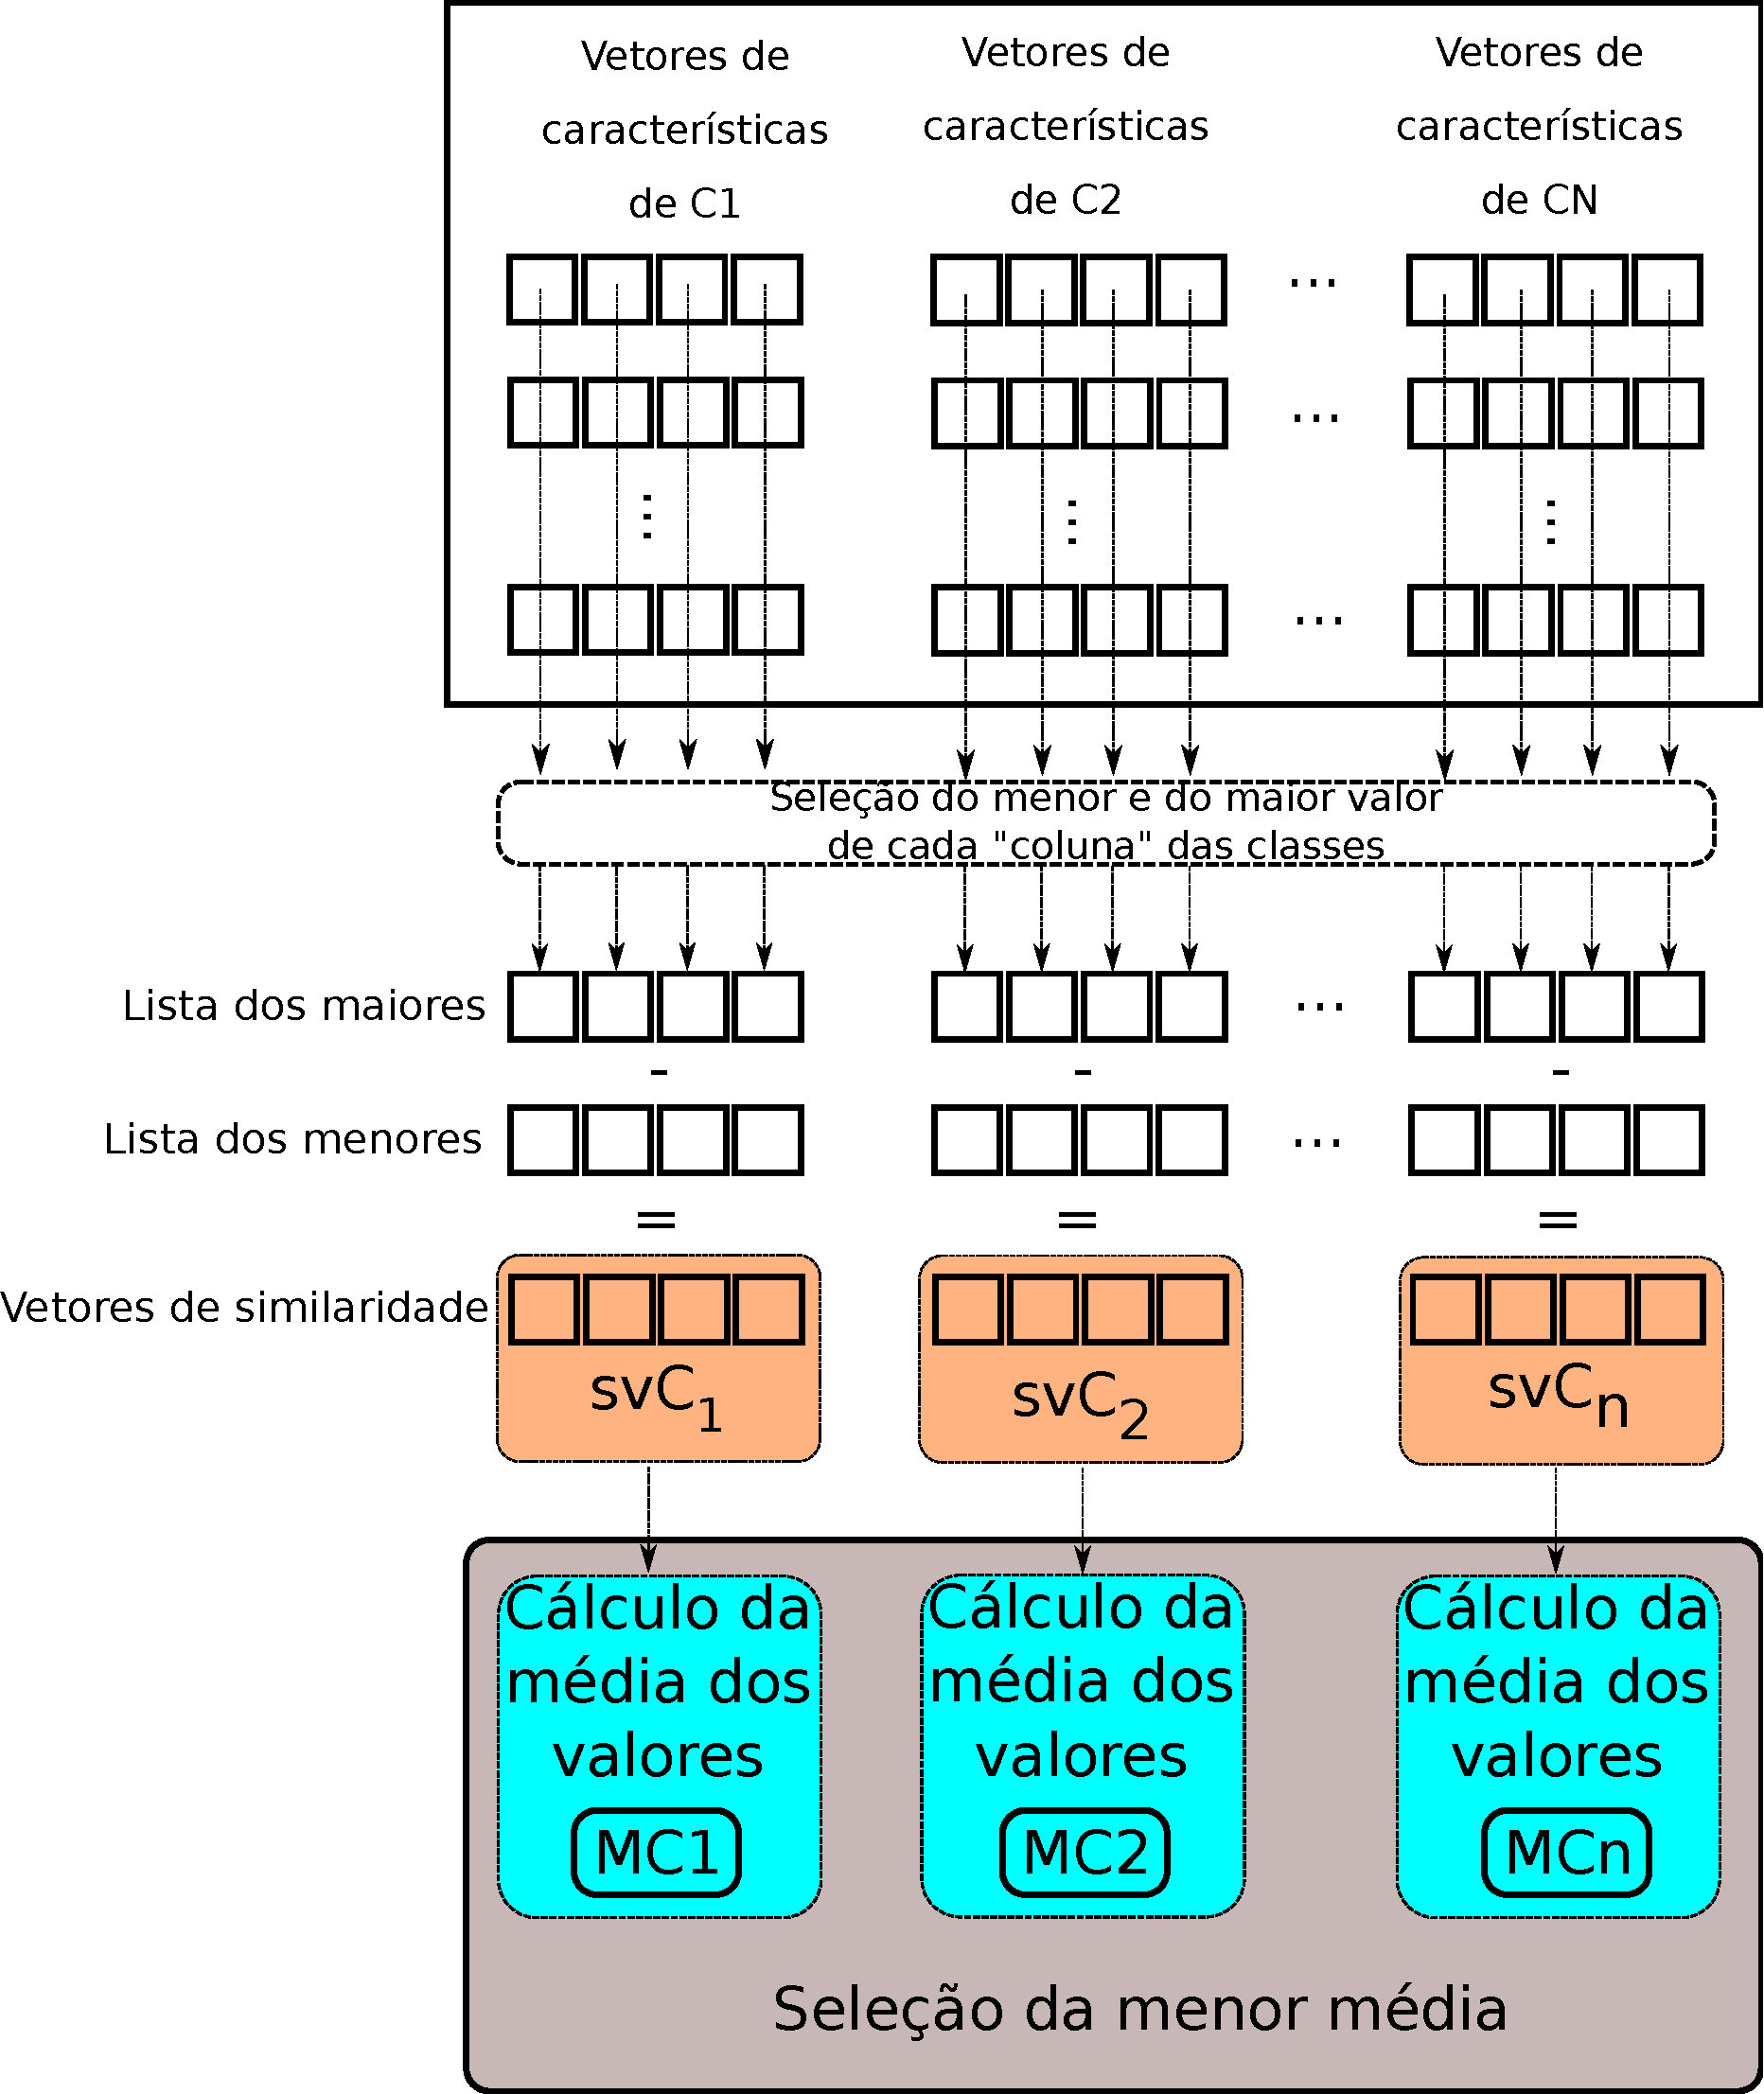
\includegraphics[width=0.6\linewidth]{images/calculoAlpha.pdf}
							\caption{Cálculo de $\alpha$}
							\label{fig:calculoalpha}
						\end{figure}
						
						\par A obtenção de $\beta$, assim como ilustrado na figura \ref{fig:betacalculation}, também se dá selecionando-se os maiores e os menores valores de cada uma das posições de todos os vetores de características de cada classe gerando assim um vetor para os valores maiores e outro para os menores.
						
						\par Na sequência se segue com o cálculo de $R$ cujo valor é a quantidade de vezes que um valor do vetor de características de uma classe se encontra no intervalo de valores maiores e menores de outra classe.
						
						\par É necessário o cálculo de $F$ que é o número máximo de sobreposições possíveis entre classes e é dado por:
						\begin{equation}
								F=N.(N-1).X.T
						\end{equation}
						onde:
						\begin{itemize}
							\item N é a quantidades de classes.
							\item X é quantidade de vetores de características por classe.
							\item T é o tamanho do vetor de características.
						\end{itemize}

						\par Finalmente, $\beta$ é calculado:
						\begin{equation}
							\beta=\dfrac{R}{F}
						\end{equation}
					
						\par Nesse ponto é importante notar que $\alpha=1$ sugere fortemente que os vetores de características de cada classe são similares e representam suas respectivas classes precisamente. Complementarmente $\beta=0$ sugere os vetores de características de classes diferentes não se sobrepõe \cite{8588433}.
						
						\begin{figure}[h]
							\centering
							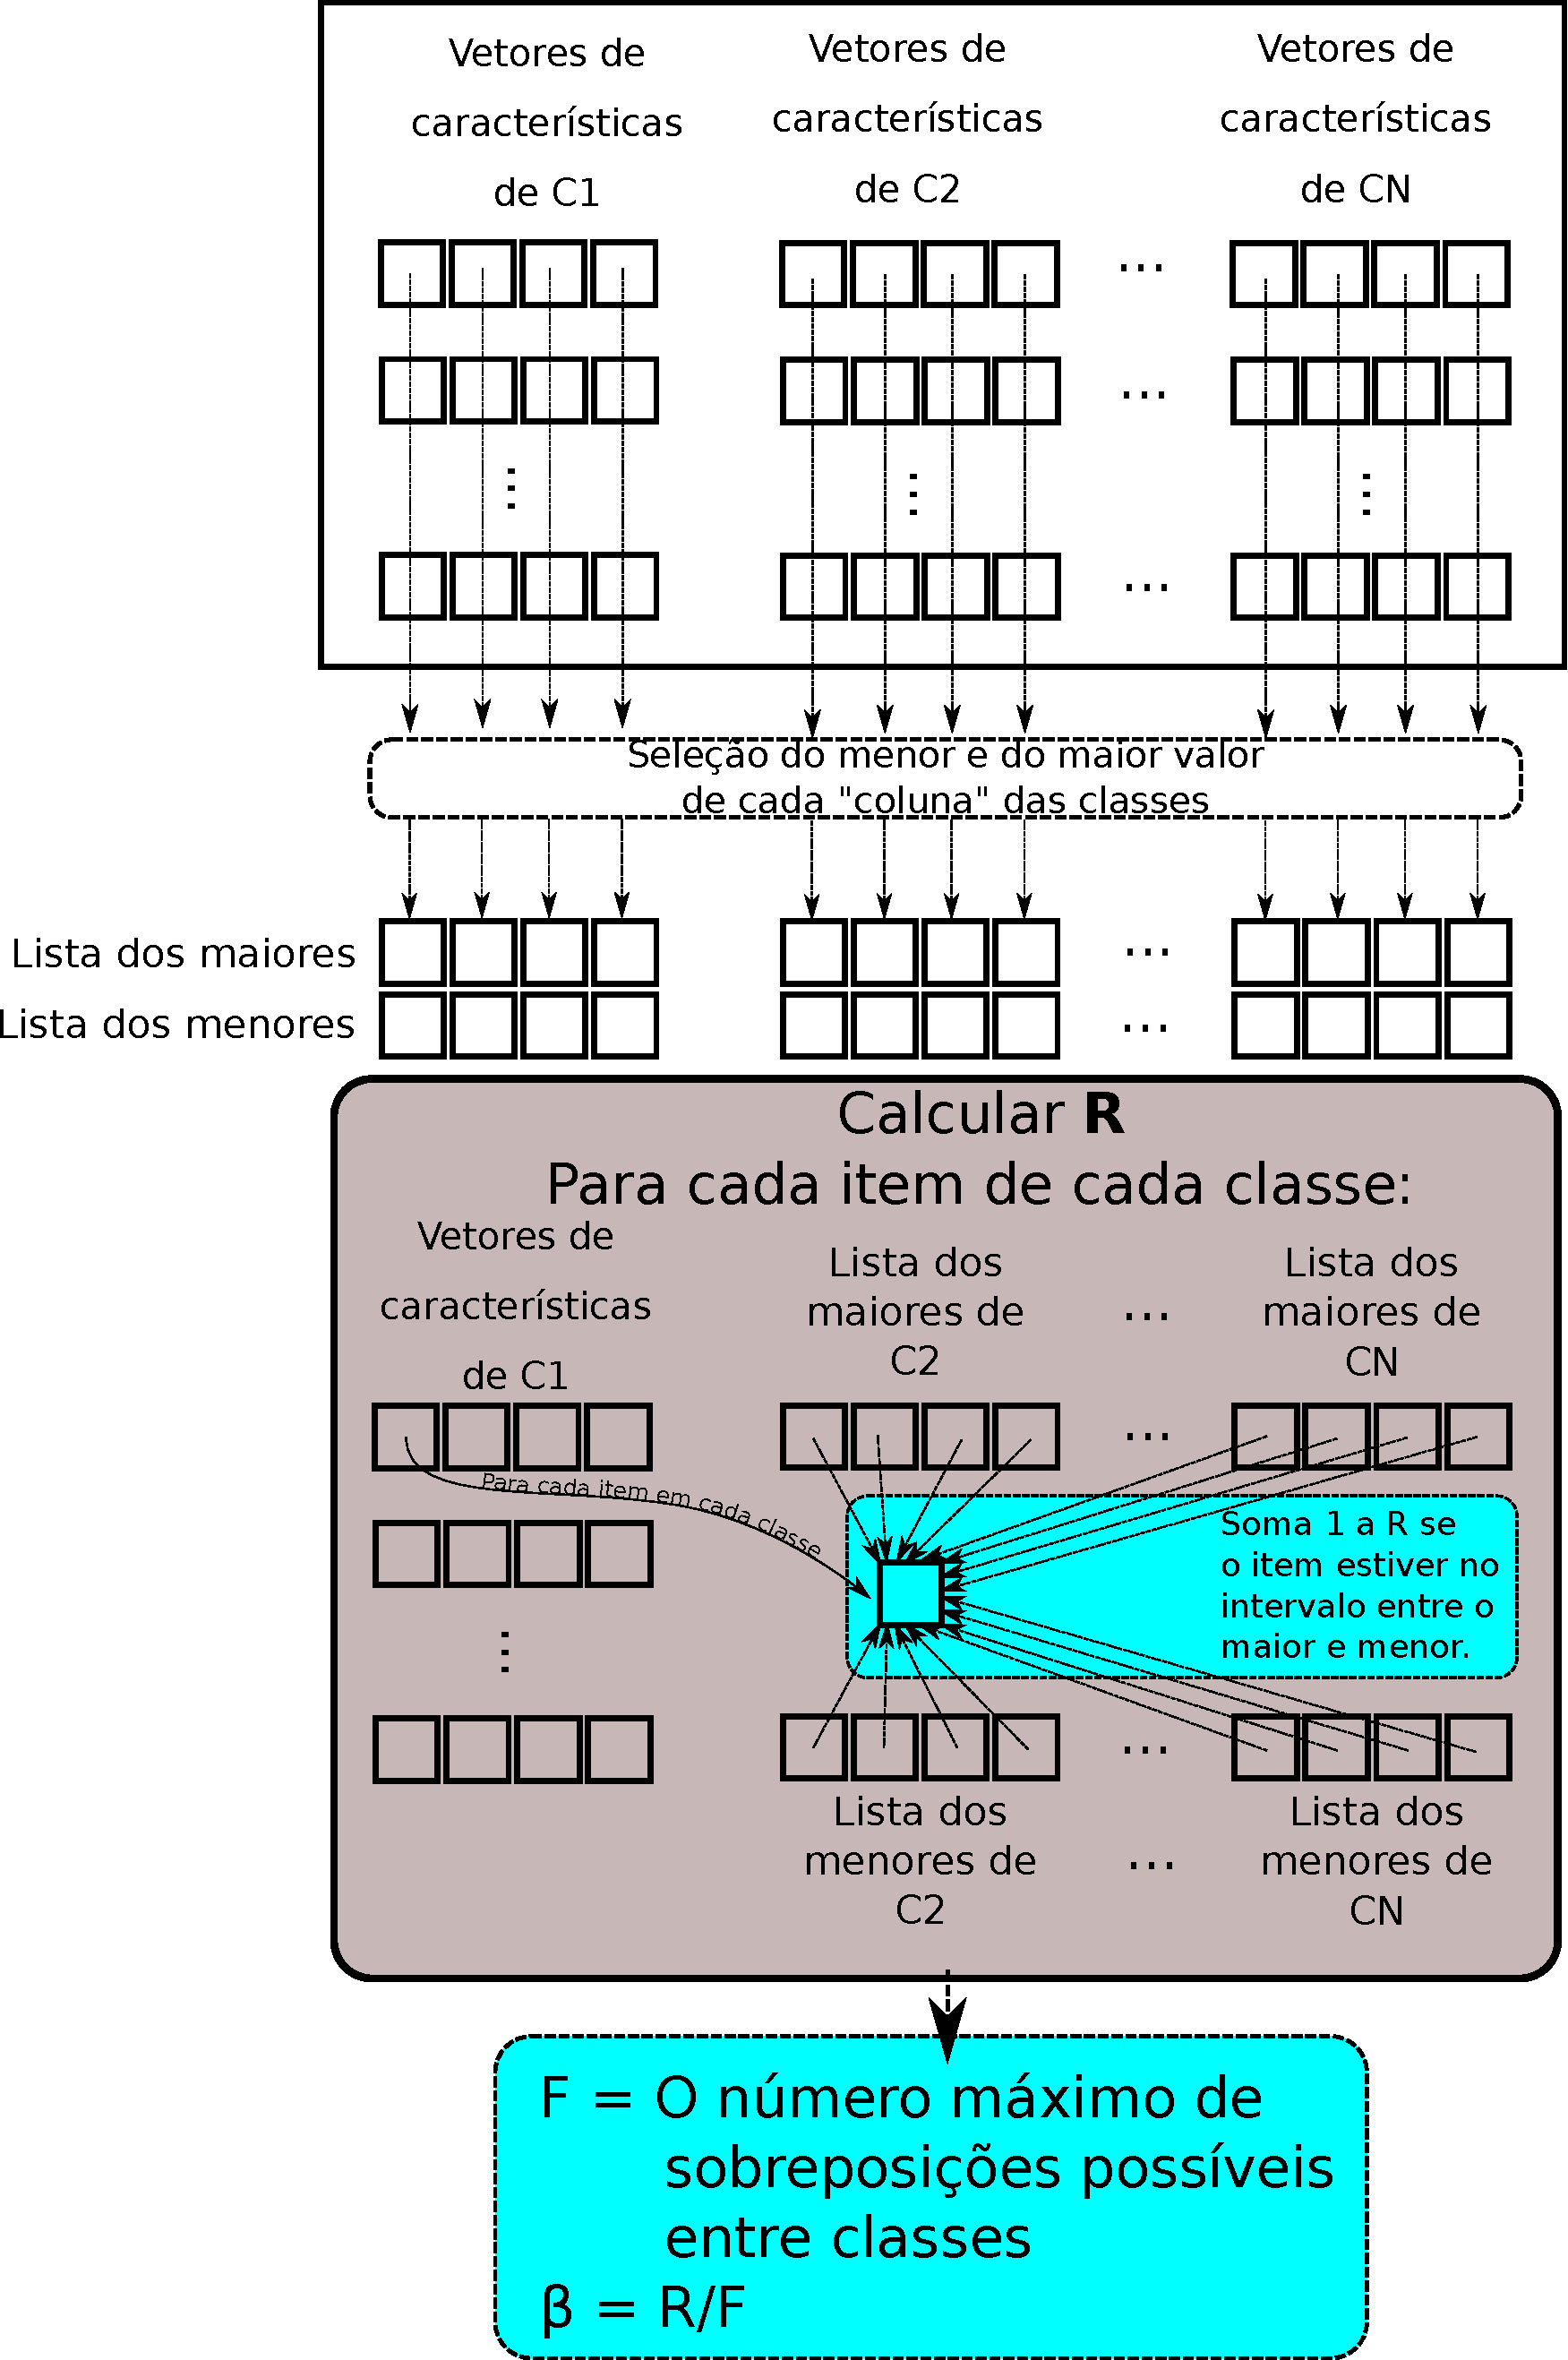
\includegraphics[width=0.55\linewidth]{images/betaCalculation.pdf}
							\caption{Cálculo de $\beta$}
							\label{fig:betacalculation}
						\end{figure}
						
						\begin{itemize}
							\item Verdade $\rightarrow$ Fé total ($\alpha = 1$) e nenhum descrédito ($\beta = 0$)
							\item Ambiguidade $\rightarrow$ Fé total ($\alpha = 1$) e descrédito total ($\beta = 1$)
							\item Falsidade $\rightarrow$ Fé nula ($\alpha = 0$) e descrédito total ($\beta = 1$)
							\item Indefinição $\rightarrow$ Fé nula ($\alpha = 0$) e descrédito total ($\beta = 0$)
						\end{itemize}
						
						\par No entanto, raramente $\alpha$ e $\beta$ terão tais valores, na maioria do tempo $0 \leqslant \alpha \leqslant 1$ e $0 \leqslant \beta \leqslant 1$, por isso, se torna necessário o cálculo do \textbf{grau de certeza}($G_1$) e do \textbf{grau de contradição}($G_2$).
						\begin{equation}
							G_1=\alpha-\beta 
						\end{equation}
						\begin{equation}
							G_2=\alpha+\beta-1 \qquad,
						\end{equation}
					onde: $-1 \leqslant G_1$ e  $1 \geqslant G_2$.

					\par Os valores de $G_1$ e $G_2$ em conjunto definem os graus entre verdade e falsidade, ou seja, $G_1=-1$ e $G_1=1$ respectivamente e também os graus entre indefinição e ambiguidade, ou seja, $G_2=-1$ e $G_2=1$ respectivamente.
					\par O plano paraconsistente para fins de visualização e maior rapidez na avaliação dos resultados como ilustrado na figura \ref{fig:paraconsistentplane} tem quatro cantos definidos:
					\begin{itemize}
						\item (-1,0) $\rightarrow$ Falsidade.
						\item (1,0) $\rightarrow$ Verdade.
						\item (0,-1) $\rightarrow$ Indefinição.
						\item (0,1) $\rightarrow$ Ambiguidade.
					\end{itemize}
					\par É importante perceber que na figura \ref{fig:paraconsistentplane} existe um pequeno círculo, este indica onde se encontram as classes nos graus explicados da listagem anterior.
					\par Para se ter ideia em que área exatamente se encontram as classes avaliadas se deve calcular as distâncias$(D)$ do ponto $P=(G_1,G_2)$ dos limites supracitados. Tal cálculo pode ser feito da seguinte forma:

					\begin{equation}
						D_{-1,0}=\sqrt{(G_1+1)^2+(G_2)^2}\qquad,
					\end{equation}
					\begin{equation}
						D_{1,0}=\sqrt{(G_1-1)^2+(G_2)^2}\qquad,
					\end{equation}
					\begin{equation}
						D_{0,-1}=\sqrt{(G_1)^2+(G_2+1)^2}\qquad,		
					\end{equation}
					\begin{equation}
						D_{0,1}=\sqrt{(G_1)^2+(G_2-1)^2}\qquad,
					\end{equation}		

					\begin{figure}[h]
						\centering
						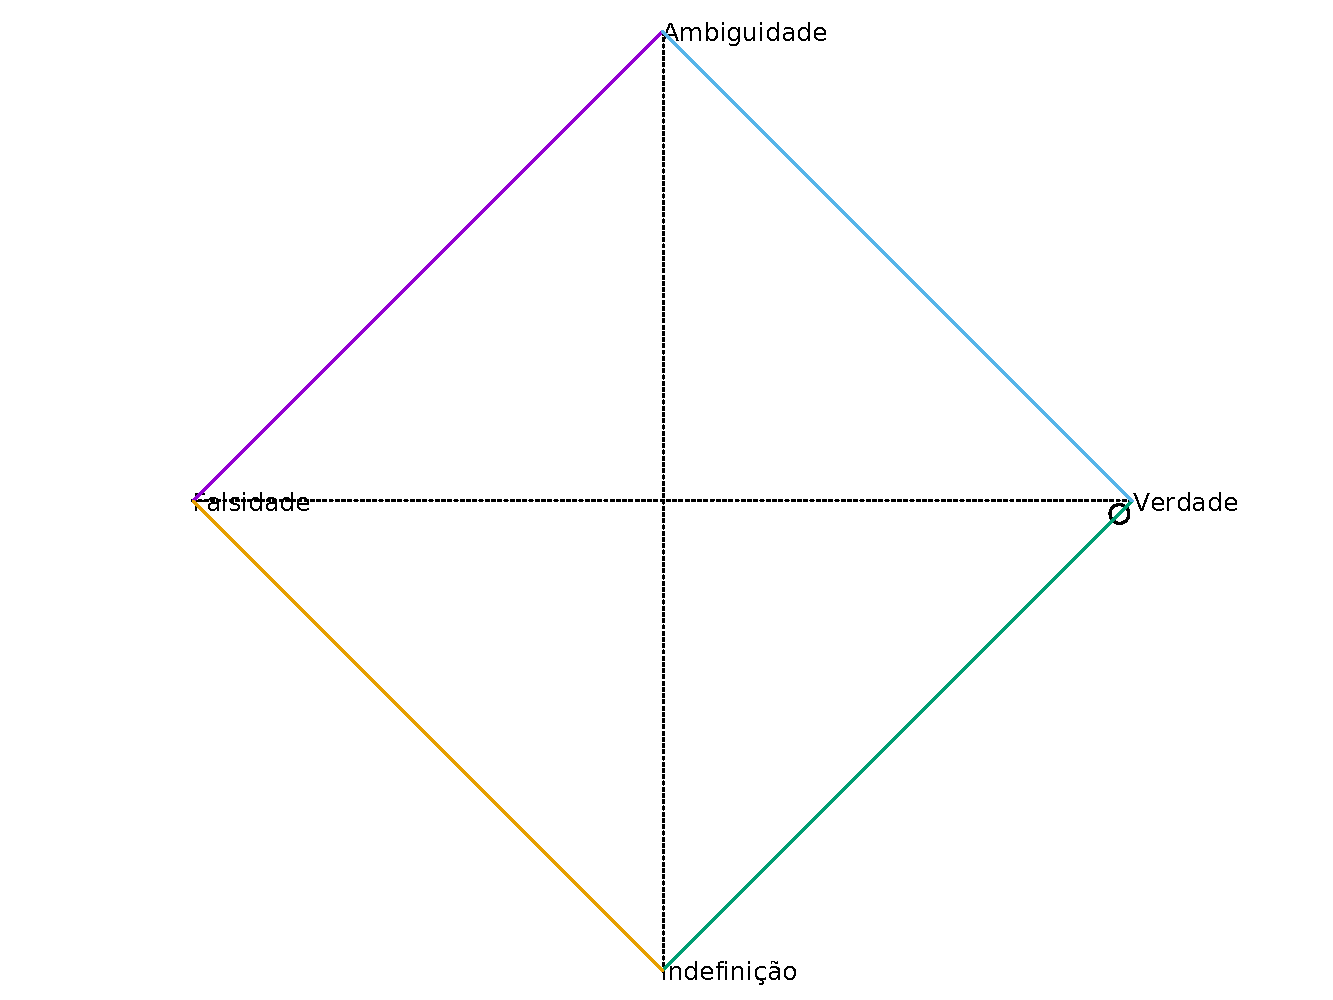
\includegraphics[width=0.69\linewidth]{images/paraconsistentPlane.pdf}
						\caption{O plano paraconsistente.}
						\label{fig:paraconsistentplane}
					\end{figure}

				\subsection{Filtros digitais wavelets}
					\par Filtros digitais \textit{wavelet} vem para suprir as deficiências em termos de janelamento de sinal apresentadas pelas transformadas de Fourier e pelas transformadas curtas de Fourier. \textit{Wavelets} contam com variadas funções filtro e tem tamanho de janela variável o que permite uma análise multirresolução \cite{Rod5254905}.
					
					\par As \textit{wavelets} proporcionam a análise do sinal de forma detalhada tanto no espectro de baixa frequência quanto no de alta frequência.
					
					\par É importante observar que, quando se trata de transformada \textit{wavelet} seis elementos estão presentes: dois filtros de análise, dois filtros de síntese e as funções ortogonais \textit{scaling} e \textit{wavelet}. No tocante a sua aplicação só a transformada direta, e não a inversa, será usada na construção dos vetores de características então os filtros de síntese, a função \textit{scaling} e a função \textit{wavelet} não serão elementos abordados aqui, pois, esses só interessariam caso houvesse a necessidade da transformada inversa. A abordagem usada será baseada nos filtros de análise digitais que proporcionarão a decomposição do sinal com o uso de filtros passa-baixa e passa-alta estritamente no domínio discreto.
		
					\par No contexto dos filtros digitais baseados em \textit{wavelets} o tamanho da janela recebe o nome de \textbf{suporte}. Janelas definem o tamanho do filtro que será aplicado ao sinal quando esse é pequeno se diz que a janela tem \textbf{um suporte compacto} \cite{robi2003}.
				
					\par Se diz que uma \textit{wavelet} tem boa \textbf{resposta em frequência} quando, na aplicação da mesma na filtragem das frequências não são causadas muitas pertubações indesejadas ao sinal, as wavelets de Daubechies se destacam neste quesito por serem \textit{maximamente planas} (Maximally-flat) nos platôs de resposta em frequência como indicado na figura \ref{fig:daubechies}.

					\begin{figure}[h]
						\centering
						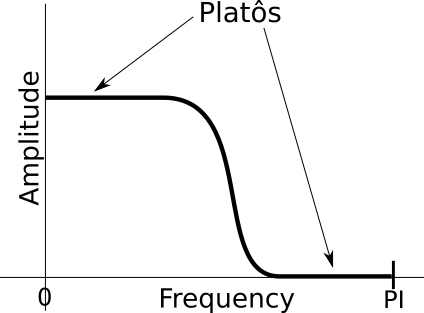
\includegraphics[width=0.3\linewidth]{images/daubechies}
						\caption{Platôs maximamente planos em um filtro digital}
						\label{fig:daubechies}
					\end{figure}

					\begin{figure}[h]
						\centering
						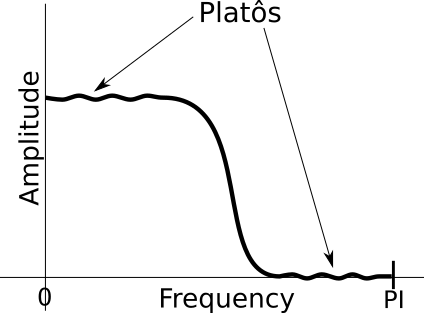
\includegraphics[width=0.3\linewidth]{images/noMaximallyFlat}
						\caption{Platôs não maximamente planos de um filtro digital}
						\label{fig:nomaximallyflat}
					\end{figure}
				
					\par Além da resposta em frequência a aplicação de um filtro digital \textit{wavelets} também pode gerar o que se chama de \textbf{resposta em fase}, esse deslocamento pode ser \textbf{linear}, \textbf{quase linear} ou \textbf{não linear}. 
					
					\begin{itemize}
						\item Na resposta em fase \textbf{linear} há o mesmo deslocamento de fase para todos os componentes do sinal.
						\item Quando a resposta em fase é \textbf{quase linear} existe uma pequena diferença no deslocamento dos diferentes componentes do sinal.
						\item Finalmente, quando a resposta é \textbf{não linear} acontece um deslocamento significativamente heterogêneo para as diferentes frequências formantes do sinal.
 					\end{itemize}
					
					\par Idealmente é desejável que todo filtro apresente boa resposta em frequência e resposta em fase linear.
					
					\begin{table}[h]
						\centering
						\begin{tabular}{|c|c|c|}
								\hline 
								\textbf{Wavelet} & \textbf{Resposta em frequência} & \textbf{Resposta em fase} \\ 
								\hline 
								Haar & Pobre &  Linear \\ 
								\hline 
								Daubechies & Quanto maior o suporte, melhor. \textit{Maximally-flat}  &  Não linear \\ 
								\hline 
								Symmlets & Quanto maior o suporte, melhor. Não \textit{Maximally-flat} & Quase linear \\ 
								\hline 
								Coiflets & Quanto maior o suporte, melhor. Não \textit{Maximally-flat} & Quase linear \\ 
								\hline 
						\end{tabular} 
						\caption{Algumas wavelets mais populares e suas propriedades}
						\label{tab:waveletsProperties}
					\end{table}
				
				\subsubsection{O algoritmo de Malat}
				\par O algoritmo de Malat torna aplicação das \textit{wavelets} no sinal em uma simples multiplicação de matrizes, o sinal que deve ser transformado se torna uma matriz linear vertical já os filtros passa-baixa e passa-alta tornam-se, nessa ordem, linhas de uma matriz quadrada que será completada segundo regras que serão mostradas mais adiante.
				\par É importante que essa matriz quadrada tenha de aresta a mesma quantidade de itens que o nosso sinal, ou seja, se o sinal tem quatro elementos então a matriz de filtros deve ser uma de 4x4.
				\par Algo interessante a se notar é que, para que seja possível a transformada wavelet, basta ter disponível o filtro passa-baixa construído a partir da \textit{mother wavelet} já que o filtro passa-alta pode ser construído a partir da ortogonalidade do primeiro.
				\par A título de exemplo considere:
				\par O filtro passa baixa baseado na wavelet Haar:
				$h[\cdot] = [\frac{1}{\sqrt{2}}, \frac{1}{\sqrt{2}}]\qquad,$
				
				\par E seu respectivo valor ortogonal:
				$g[\cdot] = [\frac{1}{\sqrt{2}}, \frac{-1}{\sqrt{2}}]\qquad,$
				
				\par Considere também o seguinte sinal:	$sinal = [1,2,3,4]\qquad.$

				\par Se o tamanho do sinal a ser tratado é quatro, ou seja, o sinal tem quatro pulsos, e se pretende-se aplicar o filtro Haar, a seguinte matriz é construída:
				\begin{equation}
					\begin{pmatrix}
						\frac{1}{\sqrt{2}}, \frac{1}{\sqrt{2}}, 0, 0\\
						\frac{1}{\sqrt{2}}, \frac{-1}{\sqrt{2}}, 0, 0\\
						0, 0, \frac{1}{\sqrt{2}}, \frac{1}{\sqrt{2}}\\
						0, 0, \frac{1}{\sqrt{2}}, \frac{1}{\sqrt{2}}\\
					\end{pmatrix} 
				\end{equation}
				\par No entanto, filtros Haar tem apenas dois valores e, necessariamente, a linha da matriz deve ter quatro itens. Para resolver este problema basta completar cada uma das linhas com zeros. A matriz é montada de forma que a mesma seja ortogonal.

				\par Montada a matriz de filtros segue-se com os cálculos da transformada:
				\begin{equation}
					\begin{pmatrix}
						\frac{1}{\sqrt{2}}, \frac{1}{\sqrt{2}}, 0, 0\\
						\frac{1}{\sqrt{2}}, \frac{-1}{\sqrt{2}}, 0, 0\\
						0, 0, \frac{1}{\sqrt{2}}, \frac{1}{\sqrt{2}}\\
						0, 0, \frac{1}{\sqrt{2}}, \frac{1}{\sqrt{2}}\\
					\end{pmatrix} 
					.
					\begin{pmatrix}
						1\\
						2\\
						3\\
						4\\
					\end{pmatrix} 
					=
					\begin{pmatrix}
						\frac{3}{\sqrt{2}}\\
						\frac{-1}{\sqrt{2}}\\
						\frac{7}{\sqrt{2}}\\
						\frac{-1}{\sqrt{2}}\\
					\end{pmatrix}
				\end{equation}
				
				\par realizada a multiplicação é necessário agora montar o sinal filtrado, isso é feito escolhendo, dentro do resultado, valores alternadamente de forma que o vetor resultante seja:

				\begin{equation}
					resultado = \Big[
					\frac{3}{\sqrt{2}},
					\frac{7}{\sqrt{2}},
					\frac{-1}{\sqrt{2}},
					\frac{-1}{\sqrt{2}}
					\Big]\qquad.
				\end{equation}
			
				\subsection{Amostragem, quantização e o formato do arquivo Wave}
					\par Serão usados arquivos no formato \textit{wave} usando \textit{pulse-code modulation} (PCM), neste esquema os dados são armazenados sem perdas. O arquivo, segundo \cite{WAVE2019}, se estrutura como o ilustrado na figura \ref{fig:wavePcmStructure}.
					
					\par A taxa de amostragem de 44100hz permite, segundo o teorema de Nyquist, que seja realizada a quantização de frequências de até 22050hz a uma resolução de 16bits.
				
					\begin{figure}[h]
						\centering
						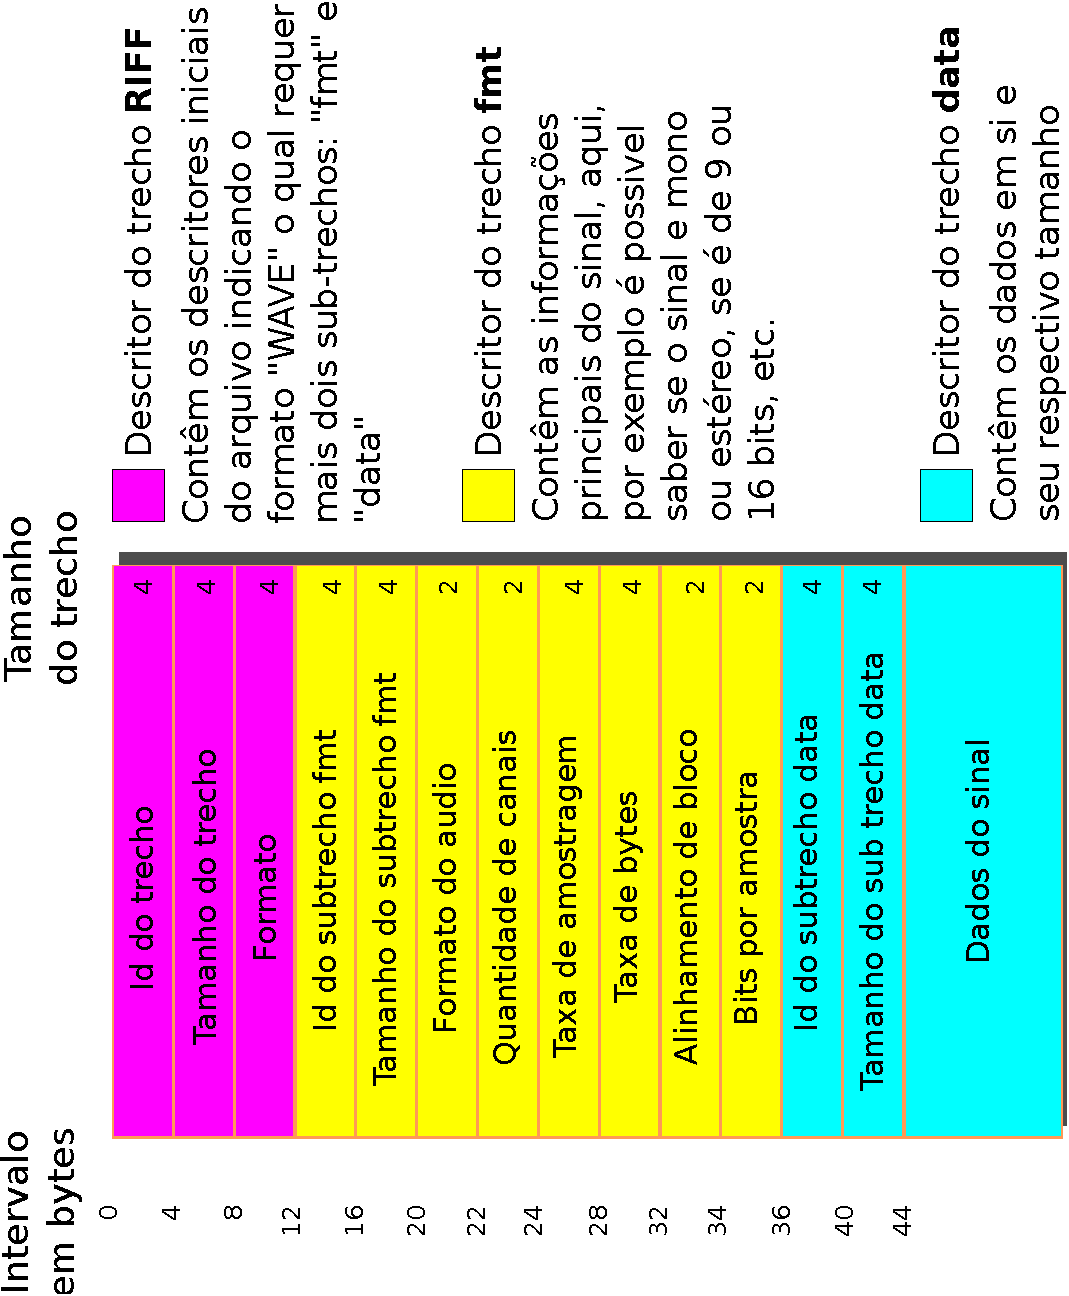
\includegraphics[width=0.45\linewidth, angle=-90]{images/wavePcmStructure.pdf}
						\caption{Estrutura do arquivo Wave}
						\label{fig:wavePcmStructure}
					\end{figure}
					
					\par A estrutura de interesse se localiza na última parte do arquivo, mais especificamente no bloco "data", aqui os dados são organizados como um grande vetor de números, cada um deles, indicando a intensidade do sinal naquele ponto.
				\subsection{Caracterização dos processos de produção da voz humana}
					\par A fala possui três grandes áreas de estudo: fisiológica (ou fonética articulatória),  acústica  (ou fonética acústica)  e  perceptual  (ou  comumente  chamada percepção  da  fala) \cite{kremer2014eficiencia}.
					\par Neste trabalho o foco será apenas na acústica, já que não serão analisados aspectos da fisiologia relacionada a voz e sim o sinal sonoro propriamente dito.
					
					\subsubsection{Vozeada versus não-vozeada}

					\par Quando da análise de voz se pode levar em consideração as partes vozeadas e/ou não-vozeadas do sinal. As partes vozeadas são aquelas produzidas com ajuda das pregas vocais, as partes não-vozeadas não tem participação desta estrutura.
					
					\subsubsection{Frequência fundamental da voz}
						\par Também conhecida como $f_0$ é o componente periódico resultante da vibração das pregas vocais, em termos de percepção se pode interpretar $f_0$ como o tom da voz (pitch) \cite{kremer2014eficiencia}.
					
						\par Vozes agudas tem um pitch alto, vozes mais graves tem um pitch baixo, a alteração do pitch durante a fala é definido como entonação.
						
						\par A frequência fundamental da voz é a velocidade na qual uma forma de onda se repete
						por unidade de tempo, ou seja, o número de ciclos vibratórios produzidos pelas pregas vocais, num segundo, sendo assim, as medidas de $f_0$ geralmente são apresentadas em Hz \cite{freitas2013avaliaccao}.
					
						\par A medição de $f_0$ está sujeita a contaminações surgidas das variações naturais de \textit{pitch} tipicas da voz humana \cite{freitas2013avaliaccao}.
						
						\par A importância de se medir $f_0$ corretamente vem do fato de que, além de carregar boa parte da informação da fala, $f_0$ é a base para construção das outras frequências, pois essas são múltiplas de $f_0$.
						
						\subsubsection{Formantes}
						
						\par \textit{O primeiro formante ($f_1$), relaciona-se à  amplificação  sonora  na  cavidade  oral  posterior  e  à  posição  da  língua  no  plano  vertical;  o segundo  formante  ($f_2$)  à  cavidade  oral  anterior  e  à  posição  da  língua  no  plano  horizontal.  O terceiro  formante  ($f_3$)  relaciona-se  às  cavidades  à  frente  e  atrás  do  ápice  da  língua;  o  quarto formante  ($f_4$),  ao  formato  da  laringe  e  da  faringe  na  mesma  altura} \cite{valencca2014analise}.

				%\subsubsection{Duvidas}
				%	\par Como o tamanho da janela funciona em wavelet? Pensei que o tamanho da janela era dado pela função de escalamento da wavelet.
				%	\par Como eu defino o tamanho da janela no algoritmo de Malat?	
				%	\par O número de sobre posições no cálculo de R é de valor ou de intervalo?

		\section{Trabalhos correlatos}
			\par No artigo \cite{Ren2019} foi apresentado um esquema de diferenciação entre a fala comum e aquela vinda de um dispositivo reprodutor. O foco da análise se dá na distorção causada pelo alto-falante segundo a energia e outras várias características do espectro do sinal. Uma base com 771 sinais de fala foi criada para cada um dos quatro dispositivos de gravação usados totalizando 3084 trechos de áudio. Uma \textit{support vector machine} (SVM) foi usada como classificador. De  acordo com os experimentos a \textit{taxa de verdadeiros positivos} é de 98,75\% e a \textit{taxa de verdadeiros negativos} é de 98,75\%.
			
			\par Em \cite{DiqunYan2019} é mostrado um método para diferenciar a voz de um locutor verdadeiro da voz gerada por sistemas usando sintetizadores baseados no \textit{modelo oculto de Markov} (HMM). SAS\cite{SAS2019} foi a escolha de base de dados. Este método usa coeficientes de características logarítmicos extraídos de wavelets que são apresentados a um classificador SVM. Os resultados obtidos tiverem, em média, mais de 99\% de acurácia.
			
			\par Usando uma decomposição por espalhamento baseada em wavelets e convertendo o resultado em coeficientes cepstrais (SCCs) o artigo \cite{7802552} cria um vetor de características que é avaliado por modelos de mistura Gaussiana (GMM). SAS e ASVspoof 2015 \cite{ASVspoof2015} foram as bases de dados escolhidas para testes. Em relação aos resultados foram usadas a \textit{taxa de falsos verdadeiros} (FAR) que representa a taxa de ocorrências falsas classificadas como verdadeiras e a \textit{taxa de falsos falsos} (FRR) que é a taxa de ocorrências verdadeiras classificadas como falsas. Aos pontos em que FAR é igual a FRR chamou-se de pontos de taxa de erros iguais e a \textit{taxa de erros iguais} (ERR) é o valor de $\dfrac{FAR}{FRR}$. Considerando isso nos experimentos foi obtida uma ERR geral de 0,18.

			\par Já em \cite{alluri2019replay} os autores usam o \textit{"Zero time windowing"} ou janelamento de tempo zero (ZTW), conceito esse que deve ser melhor entendido durante a confecção da dissertação, para, em conjunto com a análise cepstral do espectro gerado, fazer a análise do sinal. Os experimentos foram feitos usando-se a base ASVspoof 2017\cite{ASVspoof2017} com um classificador GMM, a taxa geral de ERR dos experimentos foi de 0,1475.
			
			\par Em \cite{8725688} é citado que existe uma diferença entre as propriedades espectrais da voz original e da voz gravada. No escrito são usados coeficientes cepstrais sobre os quais são aplicados uma média e uma normaliza de variância para diminuir o impacto dos ruídos na classificação. Uma GMM foi usada como classificador. A base de dados usada é a ASVspoof 2017. Quanto aos resultados se obteve uma EER geral menor que 0,1.
		
			\par A proposta de \cite{Hanilci2018} é usar sinais residuais de predição linear, para, juntamente com coeficientes cepstrais criar características que serão apresentas a um classificador GMM. Novamente, a base de dados usada foi a ASVspoof 2015 e os resultados em ERR geral foram de 5,249.

			\par Para detecção de voice spoofing  \cite{ISI:000473343500086} importa do campo de processamento de imagens o conceito de textura, para o processamento de voz esse conceito é chamado de "texturas de voz". Padrões binários locais (LBP) e seu respectivo histograma são usados para a construção do vetor de características que será avaliado por uma SVM. A base de dados usada para testes foi a ASVspoof 2015. A taxa máxima de acurácia conseguida foi de 0,7167.
			
			\par Uma abordagem que combina análise de sinal de fala usando a \textit{transformada de constante Q} (CQT) com o processamento cepstral é mostrada em \cite{TODISCO2017516}, essa técnica resulta no que se chama \textit{coeficientes cepstrais de constante Q}(CQCCs), segundo o artigo, a vantagem destes coeficientes é a resolução espectro temporal variável. As base de dados usadas foram a RedDots \cite{redDots}, ASVspoof 2015 e AVSpoof. Foram usados thês classificadores:
			\begin{itemize}
				\item DA-IICT: Uma fusão de dois classificadores GMM, sendo que um deles usa \textit{coeficientes cepstrais de frequência MEL}(MFCC) e o outro usa características CFCC-IF \cite{Patel2015}.
				\item STC \cite{7472724}.
				\item SJTU \cite{korshunov2016overview}.
			\end{itemize}			
			Na seção de experimentos são feitos testes para cada uma das bases com os seguintes resultados: ASVspoof 2015 $\rightarrow$ EER geral de 0.026; AVspoof $\rightarrow$ EER geral de 0; RedDots $\rightarrow$ EER geral de 0,185.

			\par O artigo \cite{ISI:000490497200068} propõe uma aproximação usando reverberação e as partes não vozeadas da fala, três GMMs foram definidos para a classificação, esses classificadores votam se uma ocorrência é ou não verdadeira, ganhado sempre a classificação que obtiver mais votos. A base de dado utilizada foi a ASVSpoof 2017. O sistema de avaliação de desempenho escolhido, novamente, foi o ERR e esta alcançou um valor de 2,99.
			
			\par A principal ideia de \cite{ISI:000465363900136} é capturar a amplitude instantânea vinda de flutuações instantâneas de energia. Segundo o artigo as modulações de amplitude são mais suscetíveis ao ruído inserido no sinal original por uma fonte reprodutora. O estudo usa a base de dados ASVSpoof 2017 e GMM como classificador. Os resultados apresentados chegaram a uma EER de 0.0019.

			\par No trabalho \cite{ISI:000465363900139} foram usadas as diferenças entre bandas de frequências específicas para diferenciar um sinal legítimo de um usado em ataques de falsificação. Neste trabalho é proposta a \textit{predição linear em domínio de frequência}(FDLP) juntamente com GMMs para classificação dos dados presentes na base ASVspoof  2017. Os resultados apresentados chegaram a uma EER de 0.0803.
			
			\par Em \cite{Suthokumar2018} se propõe duas novas características que visam interpretar as componentes estáticas e dinâmicas do sinal, essas características complementam as características de tempo restrito no espectro. São elas a \textit{"modulation  spectral  centroid  frequency"} e a \textit{long term spectral average}. O sistema usa como classificador um GMM juntamente com a base dados ASVSpoof 2017. Os resultados chegaram a um valor de EER de 0,0654.
			
			\par Considerando o envelopamento das amplitudes e das frequências instantâneas em cada banda estreita filtrada,  \cite{ISI:000458728700054} discute como diferenciar um sinal legítimo de um falso. A base de dados usada foi a  ASVSpoof 2015. Um GMM foi usado como classificador e, em relação ao desempenho, o método chegou a ter um EER de 0,045.

			\par Neste trabalho \cite{ISI:000392503100008} é proposto o uso do \textit{gammatone frequency cepstral coefficients}(MGFCC). O gammatone é o produto de uma distribuição gamma com um sinal senoide e é usado na construção de filtros auditivos que, neste caso, são usados para extrair características do sinal de voz. A base de dados usada foi a ASVspoof 2015. O classificador usado foi um GMM e o EER chegou a 0,02556.

			\subsection{Contextualização}
			\par No trabalho proposto para dissertação de mestrado do autor a intenção é encontrar um conjunto de características que demonstrem ser as mais disjuntas possíveis para fins de separação entre as classes, com o objetivo de melhorar a acurácia de classificadores para detecção de ataques de \textit{voice spoofing}. Caraterísticas essas com base na transformada \textit{wavelet}, devido a sua boa resolução em relação às dimensões de tempo e frequência. Essas características serão avaliadas usando a análise paraconsistente de acordo com o trabalho \cite{8588433} recentemente publicado.

		\end{myenv}

	\chapter{Cronograma para conclusão do curso de mestrado}
		\begin{myenv}{1.5}
			\par Até a presente data foram realizados os primeiros levantamentos para construção da base de dados com as vozes que serão objeto de pesquisa. Essa base conta com um total de 21 gravações originais e outras 21 de \textit{playback} gravadas de pessoas com variados gêneros e idades pronunciando os dígitos de zero a nove em Inglês. A ideia é que essa base possa crescer e abarcar boa parte dos tipos de vozes existentes na região geografica proxima ao campus da UNESP de São José do Rio Preto. Também foram estudados e implementados filtros passa-baixas e passa-altas, além de testadas metodologias de criação de vetores de características usando os intervalos espectrais pré-definidos pelas bandas MEL e BARK. 
			\par Foi melhorada a biblioteca criada e fornecida pelo orientador deste trabalho, a qual facilita a manipulação dos arquivos de áudio no formato \textit{wave}. Do mesmo modo, código-fonte para análise paraconsistente de características foi também desenvolvido e complementado com a devida documentação, a qual foi norteada por instruções recebidas do orientador.
			\par Quanto aos trabalhos futuros a tabela \ref{Cronograma} mostra o cronograma previsto.
			
			\newcommand\ytl[2]{
				\parbox[b]{10em}{
					\hfill{\color{black}\bfseries\sffamily #1}~$\cdots\cdots$~
				}
				\makebox[0pt][c]{
					$\bullet$
				}\vrule\quad \parbox[c]{4.5cm}{
				\vspace{7pt}\color{black}\raggedright\sffamily #2.\\[7pt]
				}\\
				[-3pt]
			}
		
			\begin{table}
				\centering
				\ytl{09/03 -- 31/03}{Início dos trabalhos: Coleta de dados para constituição da base de dados e estudo da base bibliográfica. Escrita da dissertação}
				\ytl{01/04 -- 15/04}{Coleta de dados para constituição da base de dados e estudo da base bibliográfica. Início dos experimentos. Escrita da dissertação}
				\ytl{16/04 -- 16/04}{Reunião de validação com o orientador}
				\ytl{17/04 -- 29/04}{Experimentos e escrita da dissertação}
				\ytl{30/04 -- 30/04}{Reunião de validação com o orientador}
				\ytl{01/05 -- 20/05}{Experimentos e escrita da dissertação}
				\ytl{21/05 -- 28/05}{Reunião de validação com o orientador}
				\ytl{29/05 -- 10/06}{Experimentos e escrita da dissertação}
				\ytl{11/06 -- 11/06}{Reunião de validação com o orientador}
				\ytl{12/06 -- 17/06}{Experimentos e escrita da dissertação}
				\ytl{18/06 -- 18/06}{Reunião de validação com o orientador}
				\ytl{19/06 -- 24/06}{Experimentos e escrita da dissertação}
				\ytl{25/06 -- 25/06}{Reunião de validação com o orientador}
				\ytl{26/06 -- 01/07}{Experimentos e escrita da dissertação}
				\ytl{02/07 -- 02/07}{Reunião de validação com o orientador}
				\ytl{03/07}{Entrega da dissertação}
				\caption{Cronograma}
				\label{Cronograma}
			\end{table}
	\end{myenv}
	\bibliography{bibliography.bib}
	\bibliographystyle{alpha}

\end{document}

